\documentclass[twocolumn]{aastex62}
\usepackage{graphicx}
\usepackage{subfigure}

\newcommand{\vdag}{(v)^\dagger}
\newcommand\aastex{AAS\TeX}
\newcommand\latex{La\TeX}

%% Reintroduced the \received and \accepted commands from AASTeX v5.2
%% Command to document which AAS Journal the manuscript was submitted to.
%% Adds "Submitted to " the arguement.
\submitjournal{ApJ}

\def\ie{{\it i.e. }}
\def\eg{{\it e.g. }}

\shorttitle{Include the Extreme Faint Galaxy in Shear Measurement}
\shortauthors{Hekun Li et al.}


\begin{document}

\title{Include the Extreme Faint Galaxy in Shear Measurement}


\correspondingauthor{Jun Zhang}
\email{betajzhang@sjtu.edu.cn}

\author{Hekun Li}
\affiliation{Department of Physics and Astronomy, Shanghai Jiao Tong University, Shanghai 200240, China}
\author{Jun Zhang*}
\affiliation{Department of Physics and Astronomy, Shanghai Jiao Tong University, Shanghai 200240, China}


\begin{abstract}



\end{abstract}


\keywords{gravitational lensing: weak-methods: data analysis}


\section{Introduction} \label{sec:intro}
noise bias, SNR threshold

precision achieved

cite the previous paper, cut and calibration to avoid bias

introduce some aspects of Fourier\_Quad and PDF\_SYM

recently, we found small bias on the faint end

multiplicative \& additive bias of these methods

\section{The Fourier\_Quad method}\label{sec:FQ}
%introduce the details of shear measurement, average approach
The Fourier\_Quad method estimates the shape of galaxy based on its 2D power spectrum. The shear estimators are defined as:
\begin{eqnarray}
\label{shear_estimator}\label{FQ_GN}
G_1&=&-\frac{1}{2}\int d^2\vec{k}(k_x^2-k_y^2)T(\vec{k})M(\vec{k})\\ \nonumber
G_2&=&-\int d^2\vec{k}k_xk_yT(\vec{k})M(\vec{k})\\ \nonumber
N&=&\int d^2\vec{k}\left[k^2-\frac{\beta^2}{2}k^4\right]T(\vec{k})M(\vec{k})
\end{eqnarray}
The $M(\vec{k})$ is the power spectrum of the galaxy image. The background and Poisson noise have been taken into account by:
\begin{eqnarray}
\label{FQ_TM}
&&M(\vec{k})=\left\vert\widetilde{f}^S(\vec{k})\right\vert^2-F^S-\left\vert\widetilde{f}^B(\vec{k})\right\vert^2+F^B\\ \nonumber
&&F^S=\frac{\int_{\vert\vec{k}\vert > k_c} d^2\vec{k}\left\vert\widetilde{f}^S(\vec{k})\right\vert^2}{\int_{\vert\vec{k}\vert > k_c} d^2\vec{k}}, \;\;\; F^B=\frac{\int_{\vert\vec{k}\vert > k_c} d^2\vec{k}\left\vert\widetilde{f}^B(\vec{k})\right\vert^2}{\int_{\vert\vec{k}\vert > k_c} d^2\vec{k}},
\end{eqnarray}
where $\widetilde{f}^S(\vec{k})$ and $\widetilde{f}^B(\vec{k})$ are the Fourier transformations of the galaxy image and a neighboring image of background noise respectively. $F^B$ and $F^S$ are the estimates of the Poisson noise power spectrum of the background noise and source images respectively. A critical wavelength, $k_c$, is required to avoid the contamination of the source power\citep{Zhang2015}. The factor $T(\vec{k})$ is the ratio of the power spectrum of the target isotropic Gaussian PSF to that of the original PSF,
\begin{equation}
T(\vec{k}) = \frac{|\widetilde{W}_{\beta}(\vec{k})|^2}{|\widetilde{W}_{PSF}(\vec{k})|^2},\quad W_{\beta}(\vec{x})=\frac{1}{2\pi \beta^2}\exp(-\frac{x^2}{2\beta^2}).
\end{equation}
It coverts the original PSF to an isotropic Gaussian PSF, so that the effect of PSF can be corrected rigorously and model-independently. The scale radius of $W_{\beta}(\vec{x})$ should be chosen sligthly larger than that of $W_{PSF}(\vec{x})$ to avoid the singularities in the factor $T(\vec{k})$. 

The ensemble averages of the shear estimators recover the shear signal to its second order in accuracy\citep{Zhang2015}:
\begin{eqnarray}
\label{mean}
\frac{\left\langle  G_1\right\rangle }{\left\langle  N\right\rangle }=g_1+O(g_{1,2}^3),\;\;\;\frac{\left\langle  G_2\right\rangle }{\left\langle  N\right\rangle }=g_2+O(g_{1,2}^3).
\end{eqnarray}
This is the average approach for shear recovery. The ensemble average should be applied to the denominator and numerator respectively. \cite{Zhang2015} have shown the appealing advantage of Fourier\_Quad that including the extreme faint sources or even point sources would not bias the shear measurement. However, a certain signal-to-ratio threshold is required for the shear measurement in many other methods.

To approach the lower statistical error bound, \cite{Zhang2017} propose a new shear recovery method in the Fourier\_Quad framework which is called the PDF\_SYM approach. It estimates the unbiased shear signal by symmetrizing the probability distribution function (PDF) of the shear estimators. \cite{Zhang2017} show that the PDF of $G_{1/2} - \hat{g}_{1/2}(N\pm U)$ would be maximally symmetrical respect to zero if the shear estimate, $\hat{g}_{1/2}$, is the true one (see the Ref. for more details). The PDF\_SYM approach needs two additional shear estimators, $U$ and $V$.
\begin{eqnarray}\label{FQ_UV}
U = -\frac{\beta^2}{2}\int d^2\vec{k}(k_x^4 - 6k_x^2k_y^2 + k_y^4)T(\vec{k})M(\vec{k}), \\ \nonumber
V = -2\beta^2\int d^2\vec{k}(k_x^3k_y - k_xk_y^3)T(\vec{k})M(\vec{k}).
\end{eqnarray}
The $V$ term is kept for the rotation with $U$. 

Unlike the weighted sum of shear estimators used by the other methods, the PDF\_SYM approach includes the full PDF of the shear estimators and do not weight down the faint sources. Therefore, it could make full use of the additional information from faint sources to achieve a lower statistical error. The PDF\_SYM approach would be a promising method for shear recovery in the Fourier\_Quad framework.




\section{To achieve sub-percent precision on the extreme low SNR end}
Recently, we find the PDF\_SYM approach would be biased by the very faint galaxies. The multiplicative bias is about $1\%$ level when the SNR decreases to about $10$. If the PSF has some anisotropy ($e \sim 0.1$), we could also find significant additive bias ($\sim 6\times 10^{-4}$) at the same SNR level. Figure \ref{fig:pts_mc} shows the multiplicative and additive bias of different SNR sample. While $\sim 1\%$ bias has been found at the very faint end, it would not be a serious problem for the real measurement that includes samples from faint to bright. The result of a more realistic simulation will be shown in Section \ref{sec:improve}. The parameters of image simulation 

\begin{figure*}[htbp]
	\centering
	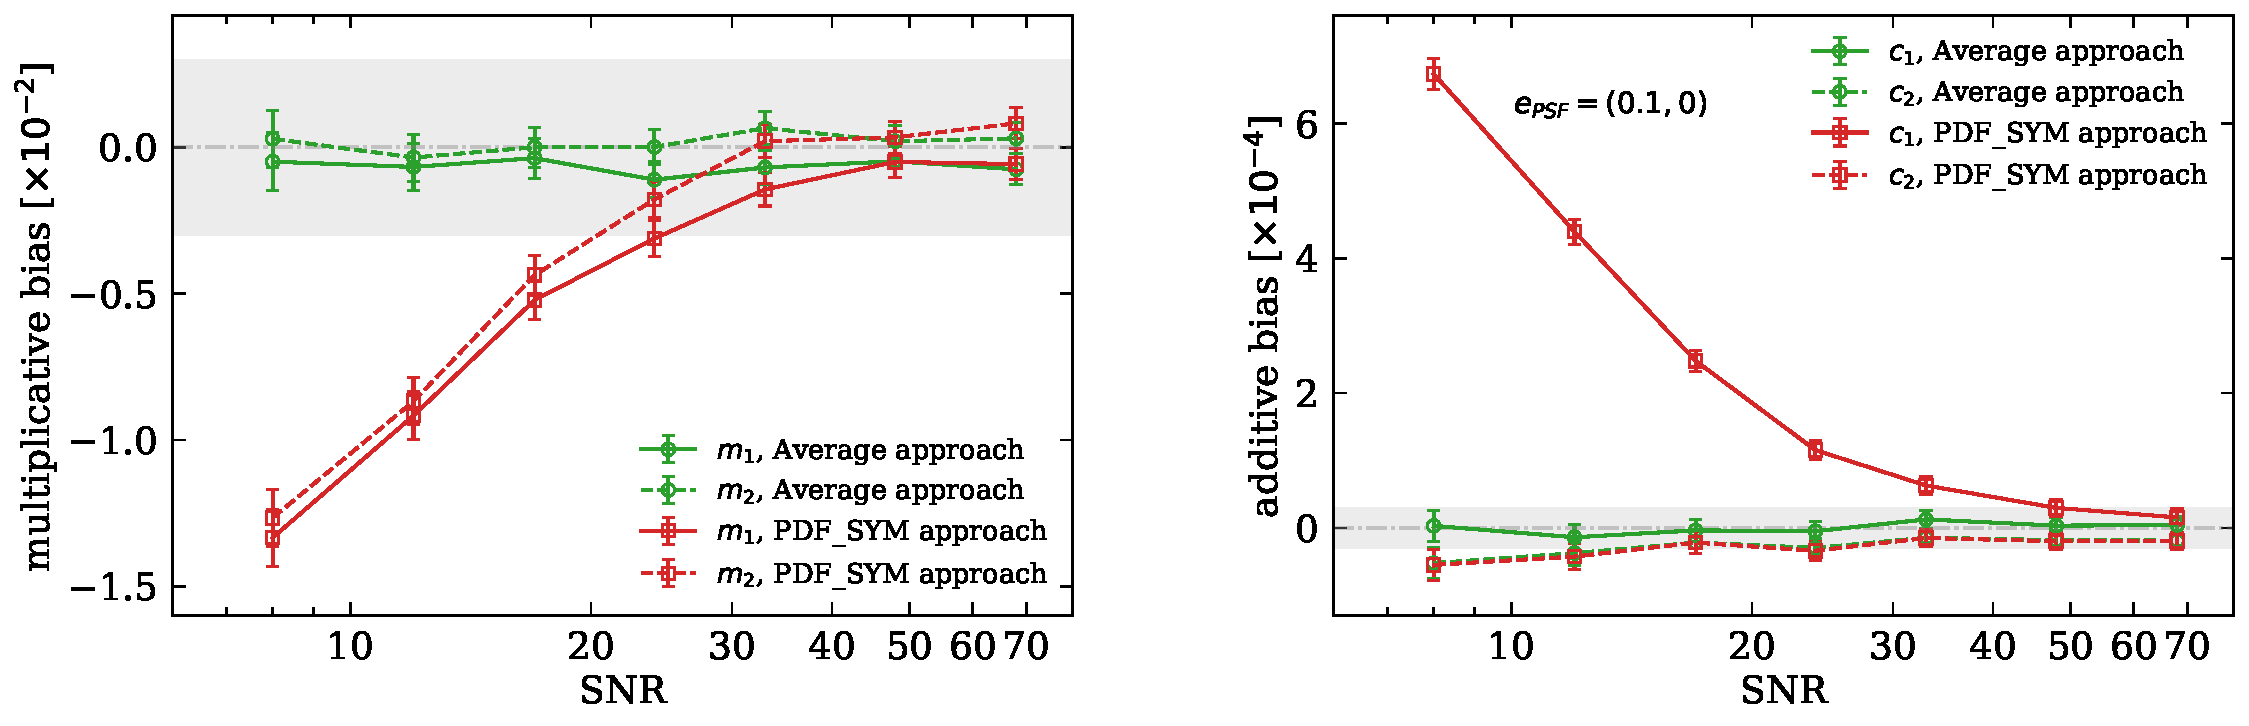
\includegraphics[width=0.9\linewidth]{figures/pts_sample_mc.pdf}
	\caption{The multiplicative and additive bias measured from the galaxy of different SNR level. The shaded region in the left (right) panel is between $\pm 3\times 10^{-3}$ ($\pm 3\times10^{-5}$) which is the fluctuation allowed in the Fourier\_Quad method. }\label{fig:pts_mc}
\end{figure*}

\subsection{Image simulation}
The real galaxies consist of millions of stars which are the point sources. We generate the galaxies with the random walk method. Each galaxy is made of a number of points. In this method, we let a random walker wanders in a circular region from image center. The points of galaxy are the collection of positions of each step the walker has reached. The merit of random walk method includes precise shape distortion, less computational cost and efficient PSF convolution.

We use Moffat PSF in the simulation. 
\begin{eqnarray}
I(r) \propto \left[1+\left(\frac{r}{r_d}\right)^2\right]^{-3.5}H(r_c-r).
\end{eqnarray}
$H(r_c-r)$ is the Heaviside step function, $r_d$ is the scale length and $r_c$ is set to 4 times $r_d$. The stamp size is $44\times44$. 40 shear pairs random choice on the $g_1-g_2$ plane are used. $10^7$ galaxies are generated for each shear point.


\subsection{Bias due to the mixture of source and noise}
To reveal the origin of the bias, let us start from the components of galaxy image. It can be written as a sum of source and noise image, \ie$f^S(\vec{x}) = f^G(\vec{x}) + f^N(\vec{x})$. Therefore, the modified power spectrum of galaxy image, $M(\vec{k})$, can be rewritten as 
\begin{eqnarray}
M(\vec{k}) = F(\vec{k}) + C(\vec{k}) + \Delta N(\vec{k}).
\end{eqnarray}
$F(\vec{k})$ is the power spectrum of the noise free galaxy image, $\left\vert\widetilde{f}^G(\vec{k})\right\vert^2$. $C(\vec{k})$ is the mixture term of the Fourier transform of source and that of the background noise. $\Delta N(\vec{k})$ is the noise power spectrum residual. 
\begin{eqnarray}
&C(\vec{k})& = \widetilde{f}^{G*}(\vec{k})\widetilde{f}^N(\vec{k}) + \widetilde{f}^{G}(\vec{k})\widetilde{f}^{N*}(\vec{k}),\\ \nonumber
&\Delta N(\vec{k})& = \left\vert\widetilde{f}^N(\vec{k})\right\vert^2 -\left\vert\widetilde{f}^B(\vec{k})\right\vert^2.
\end{eqnarray}
We have dropped the estimate of the Poisson noise power spectrum, $F^S$ and $F^B$, because they are not import here. 

It should be noted that these three parts of $M(\vec{k})$ are also 2D images from which we can apply the operations defined in Section \ref{sec:FQ} to obtain the shear estimators. Furthermore, the bias origin could be found out by using the combination of shear estimators from different part in $M(\vec{k})$. Figure \ref{fig:pts_componets} shows that the mixture of Fourier transform of the galaxy image and that of the background noise image, $C(\vec{k})$, causes both multiplicative and additive bias in the measurement.
\begin{figure*}[htbp]
	\centering
	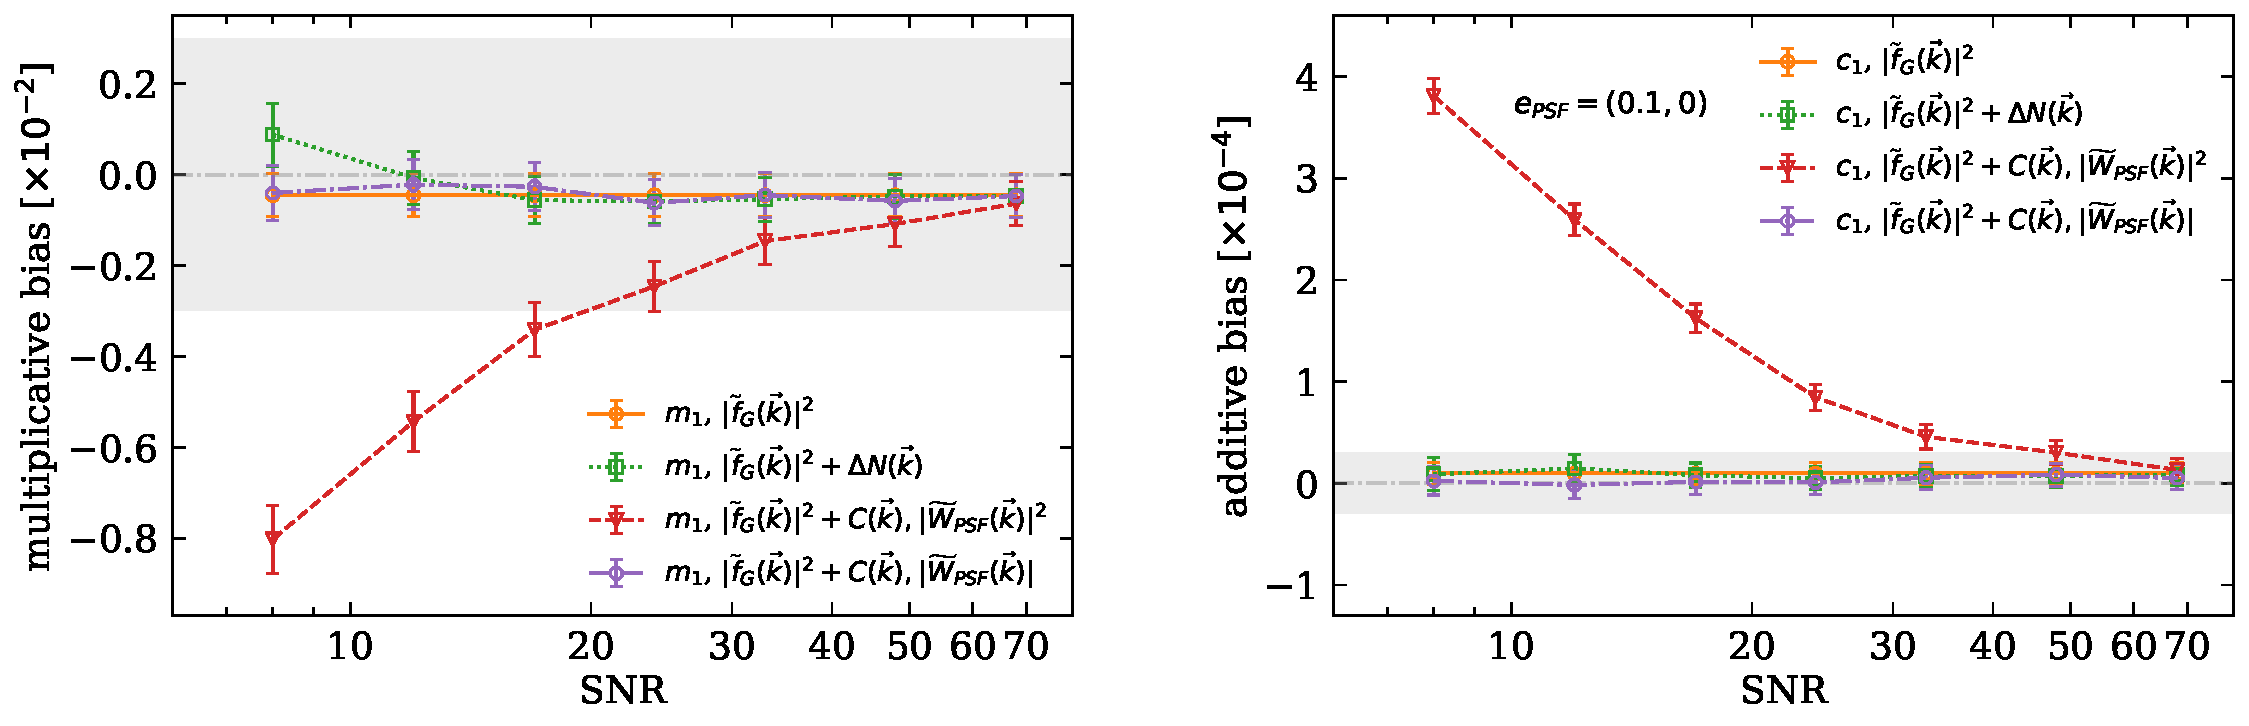
\includegraphics[width=0.9\linewidth]{figures/pts_sample_components.pdf}
	\caption{The multiplicative and additive bias measured from different components of the power spectrum of noisy galaxy image. Orange curves: measured from the power spectrum of noise free image, $F(\vec{k})$. Red curves: measured from the combination of the noise free part, $F(\vec{k})$, and the Fourier transform mixture, $C(\vec{k})$. Green curves: measured from the combination of noise free part and the noise power spectrum residual, $\Delta N(\vec{k})$.}\label{fig:pts_componets}
\end{figure*}

bias origin, the crossing term $\rightarrow$ bias from the inappropriate PSF deconvolution for the crossing term

figure of the effects of crossing term to the noise free image

figure of comparison of bias from the original PSF deconvolution and the appropriate PSF deconvolution for the crossing term

use the formulae to show the details of origin of the bias, m\&c

\subsection{Improvement to the sub-percent precision}\label{sec:improve}
use the formulae to show the way of correction by new crossing term

introduce the method to obtain the estimated crossing term \& apply to the simulated data

figure of the results of correction, random walk galaxies, SNR\_1 $\sim$ SNR\_n

figure of the same results from the Galsim galaxies, SNR\_1 $\sim$ SNR\_n

figure of a more realistic simulation, galaxies form faint to bright, separate the bright and faint sample

\section{conclusion}



\begin{thebibliography}{}

\bibitem[Rowe et al.(2015)]{Rowe2015}Rowe B, Jarvis M, Mandelbaum R, et al. \ 2015, A\&C, 10, 121

\bibitem[Zhang(2008)]{Zhang2008} Zhang J. \ 2008, \mnras, 383, 113


\bibitem[Zhang et al.(2015)]{Zhang2015} Zhang J, Luo W \& Sebastien F. \ 2015 \jcap, 1, 24

\bibitem[Zhang et al.(2017)]{Zhang2017} Zhang J, Zhang P, Luo W. \ 2017, \apj, 834, 8

\end{thebibliography}

\end{document}

% End of file `sample62.tex'.
